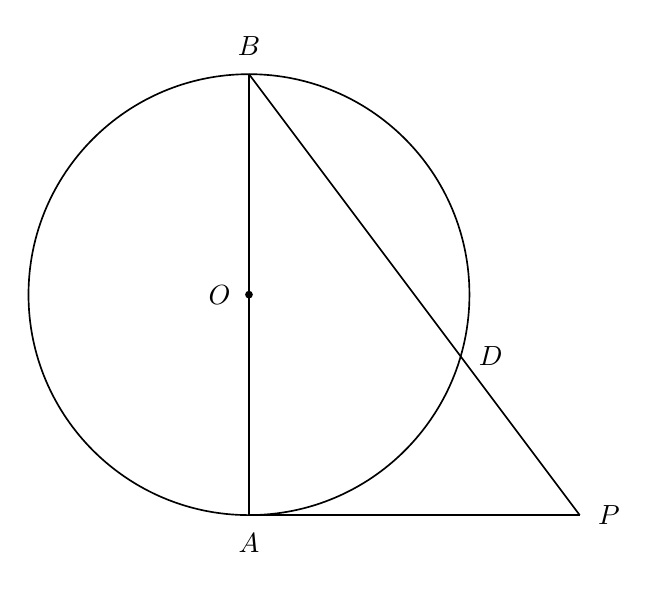
\begin{tikzpicture}[x=1cm,y=1cm,line width=.6pt,font=\normalsize]
\coordinate (O) at (0,0);
\coordinate (A) at (0,-2.8);
\coordinate (B) at (0,2.8);
\coordinate (P) at (4.2,-2.8);
\coordinate (D) at (2.688,-0.784);
\draw (O) circle[radius=2.8cm];
\draw (A)--(B);
\draw (A)--(P);
\draw (B)--(P);
\fill (O) circle[radius=1.4pt];
\node[left=3pt] at (O) {$O$};
\node[below=3pt] at (A) {$A$};
\node[above=3pt] at (B) {$B$};
\node[right=3pt] at (P) {$P$};
\node[right=3pt] at (D) {$D$};
\end{tikzpicture}
